\section{Career Paths}
\label{sect:career-paths}
The goal of the career paths module is to generate data, such that a web user
interface could generate a graph of the career paths taken to reach the
specified career goal.  The vertex edge transitions along with the edge
transition frequencies are returned to the user interface as objects.  Additionally,
the vertex ordering and information about each individual vertex is also returned in
an object.  This information can then be used to generate a graph
depicting various ways of achieving a career goal.  

An example of one of these graphs depicted in Figure~\ref{fig:nodal map}, which
shows various interconnected vertices that eventually arrive at the goal vertex.  The vertices
are arranged such that the user most likely travels from left to right, but the
occasional infrequently traveled transition may flow in the reverse direction. 
In this example, the frequency that the edge is traveled is depicted through
line thickness.  This is done so that a visual representation is available to
show approximately how many of the total returned users transition from one
vertex to another.  A dotted line would be the least frequently traveled edge,
then a dashed line, a thin line, and finally the most frequently traveled edge
would be the thick line. 

Each vertex would then be able to display the individual vertex information upon
user request; either through clicking on the vertex or through some other user
action.  Note, that ProGENitor does not limit the method in which the user
interface is displayed; it simply passes back statistical information about the
vertices, the transitions between each vertex, and the individual data about
each vertex.  It is up to the web user interface developer to determine how the
end product is rendered.


\usetikzlibrary{shapes,arrows,chains,decorations.markings}

\begin{figure}[H]
	\centering
  
% Start the picture
\resizebox {125mm} {!} {
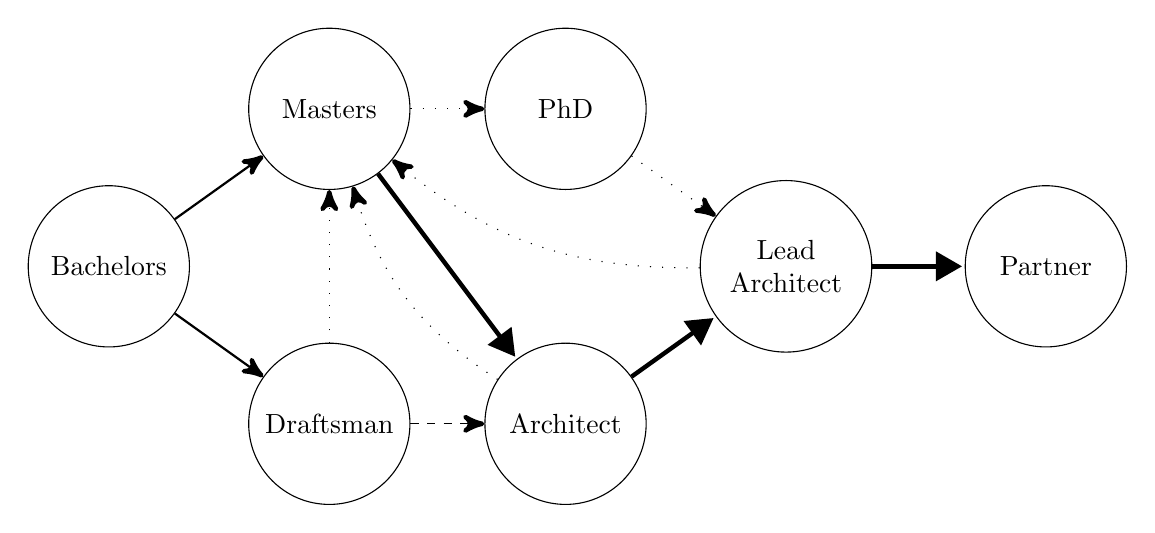
\begin{tikzpicture}[%
    >=triangle 60,              % Nice arrows; your taste may be different
    start chain=going below,    % General flow is top-to-bottom
    node distance=3mm and 28mm, % Global setup of box spacing
    every join/.style={norm},   % Default linetype for connecting boxes
    ]
% ------------------------------------------------- 
% A few box styles 
% <on chain> *and* <on grid> reduce the need for manual relative
% positioning of nodes
\tikzset{
  base/.style={draw, on chain, on grid, align=center, minimum height=2ex},
  node/.style={base, circle, text width=5em},
  % Connector line styles for different parts of the diagram
  norm/.style={->, draw},
  tn/.style={->,>=stealth',shorten >=1pt, loosely
  dotted,decoration={markings,mark=at position 1 with {\arrow[ultra thick]{>}}}, postaction={decorate}
  },
  nm/.style={->,>=stealth',shorten >=1pt,dashed,decoration={markings,mark=at
  position 1 with {\arrow[ultra thick]{>}}}, postaction={decorate}
  },
  to/.style={->,>=stealth',shorten >=1pt,thick,decoration={markings,mark=at
  position 1 with {\arrow[ultra thick]{>}}}, postaction={decorate}
  },
  tk/.style={->,shorten >=1pt,ultra thick},
  it/.style={font={\small\itshape}}
}
% -------------------------------------------------
% Start by placing the nodes
\node [node] (a) {Bachelors};
% Use join to connect a node to the previous one 
\node [node, right = of a, yshift=20mm] (b) {Masters};
\node [node, right = of a, yshift=-20mm] (c) {Draftsman}; 
\node [node, right = of b, xshift=2mm](d) {PhD};
\node [node, right = of c, xshift=2mm](e) {Architect};
\node [node, right = of e, yshift=20mm](f) {Lead Architect};
\node [node, right = of f, xshift=5mm](g) {Partner};

\draw[to] (a) to (c);%Bachelors,Draftsman,4
\draw[tn] (c) to (b);	%Draftsman,Masters,1
\draw[tk] (b) to (e);	%Masters,Architect,7
\draw[tk] (e) to (f);	%Architect,Lead Architect,7
\draw[tk] (f) to (g);	%Lead Architect,Partner,7
\draw[to] (a) to (b);	%Bachelors,Masters,5
\draw[tn] (b) to (d); %Masters,PhD,0
\draw[tn] (d) to (f);	%PhD,Lead Architect,0
\draw[nm] (c) to (e);	%Draftsman,Architect,2
\draw[tn] (e) to [bend left=20] (b);	%Architect,Masters,0
\draw[tn] (f) to [bend left=20] (b);	%Lead
% Architect,Masters,0

% -------------------------------------------------
\end{tikzpicture}
}

	\caption{Career Path Graph}
	\label{fig:nodal map}
\end{figure}

\subsection{Graph Edges}
The graph edges portion of code finds all of the vertices that
users pass through and the order at which they pass through them.  It then
tallies the number of times all of the users pass along each transition
path to allow for the career path graph to depict not only the point to point
connections, but also how frequently that edge is traveled.  The high level
process to generate this graph interconnection data is depicted in
Figure~\ref{fig:node interconnect}.


\usetikzlibrary{shapes,arrows,chains}

\begin{figure}[H]
	\centering
% Start the picture
\resizebox {!} {110mm} {
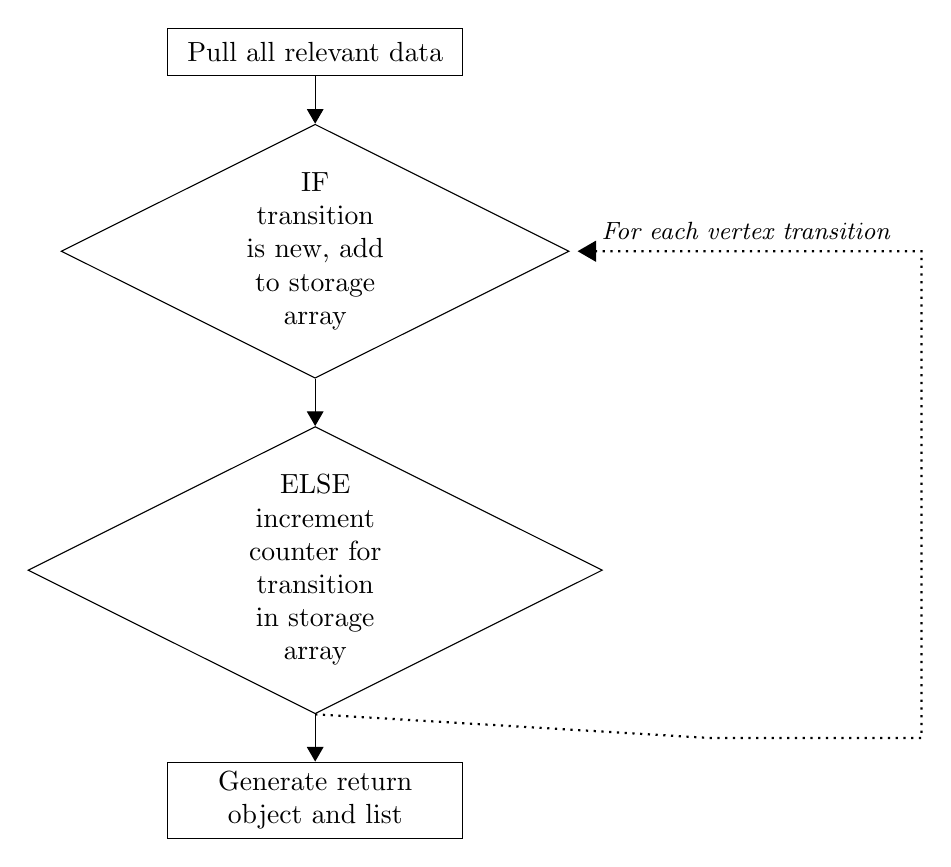
\begin{tikzpicture}[%
    >=triangle 60,              % Nice arrows; your taste may be different
    start chain=going below,    % General flow is top-to-bottom
    node distance=6mm and 60mm, % Global setup of box spacing
    every join/.style={norm},   % Default linetype for connecting boxes
    ]
% ------------------------------------------------- 
% A few box styles 
% <on chain> *and* <on grid> reduce the need for manual relative
% positioning of nodes
\tikzset{
  base/.style={draw, on chain, on grid, align=center, minimum height=4ex},
  proc/.style={base, rectangle, text width=10em},
  test/.style={base, diamond, aspect=2, text width=5em},
  % Connector line styles for different parts of the diagram
  norm/.style={->, draw},
  it/.style={font={\small\itshape}}
}
% -------------------------------------------------
% Start by placing the nodes
\node [proc] (p0) {Pull all relevant data};
% Use join to connect a node to the previous one 
\node [test, join] (t1) {IF transition is new, add to storage array};
\node [test, join] (t2) {ELSE increment counter for transition in storage
array}; 
\node [proc, join](p1) {Generate return object and list};

\draw [->, dotted, thick, shorten >=1mm]
  (t2.south) -- ++(50mm,-3mm)  -- ++(27mm,0) 
  |- node [black, near end, yshift=0.75em, it]
    {For each vertex transition} (t1);

% -------------------------------------------------
\end{tikzpicture}
}
	\caption{High Level Graph Edge Generation}
	\label{fig:node interconnect}
\end{figure}

\noindent The process flow in defining and counting these edges is listed
in detail below:

\begin{description}
    \item[Graph Edge Generation:]
\end{description}
\begin{enumerate}
  \item For each ID passed to edge generation module:
  \begin{enumerate}
    \item Pull job data and add it to the vertices list.
    \item Pull education data and add it to the vertices list.
    \item Set Min equal to Max Integer and Max equal to MIN Integer.
    \item For each element of the vertices list:
    \begin{enumerate}
      \item If date of data for element of vertices is less than Min and more
      than Max, store the data and set Min equal to date of data.
      \item After all elements of vertices list considered, add stored data
      to user list and set Max equal to Min.
  	\end{enumerate}
  	\item For each element of user list:
  	\begin{enumerate}
  	  \item If A is NULL, set A equal to user element vertex name.
  	  \item Else set B equal to A and set A equal to user element vertex name.
  	  \item If edges list is empty, add B,A,1 to edges list.
  	  \item Else check if B,A exists in the edges list:
  	  \begin{enumerate}
  	    \item If it exists, increment the counter of the row.
  	    \item If it does not exist, add B,A,1 to the edges list.
  	  \end{enumerate}
  	\end{enumerate}
  \end{enumerate}
  \item Push edges list containing all graph transitions and transition
  counts to an object containing an array.
  \item Return both the list and the object.
\end{enumerate}

\subsection{Vertex Ordering}
The vertex ordering portion of code sorts the vertices such that the major
transitions flow in order from start to finish. It does this so that the flow
of transitions can be graphed in a manner that is not overly confusing. 
Figure~\ref{fig:node ordering} shows the high level process that the code
follows to generate the vertex groupings.  These groupings can then be fed to
the end user interface to order the vertices in a fashion that shows the typical
flow of careers that reach the destination goal.

\usetikzlibrary{shapes,arrows,chains}

\begin{figure}[H]
	\centering
	\resizebox {!} {145mm} {
% Start the picture
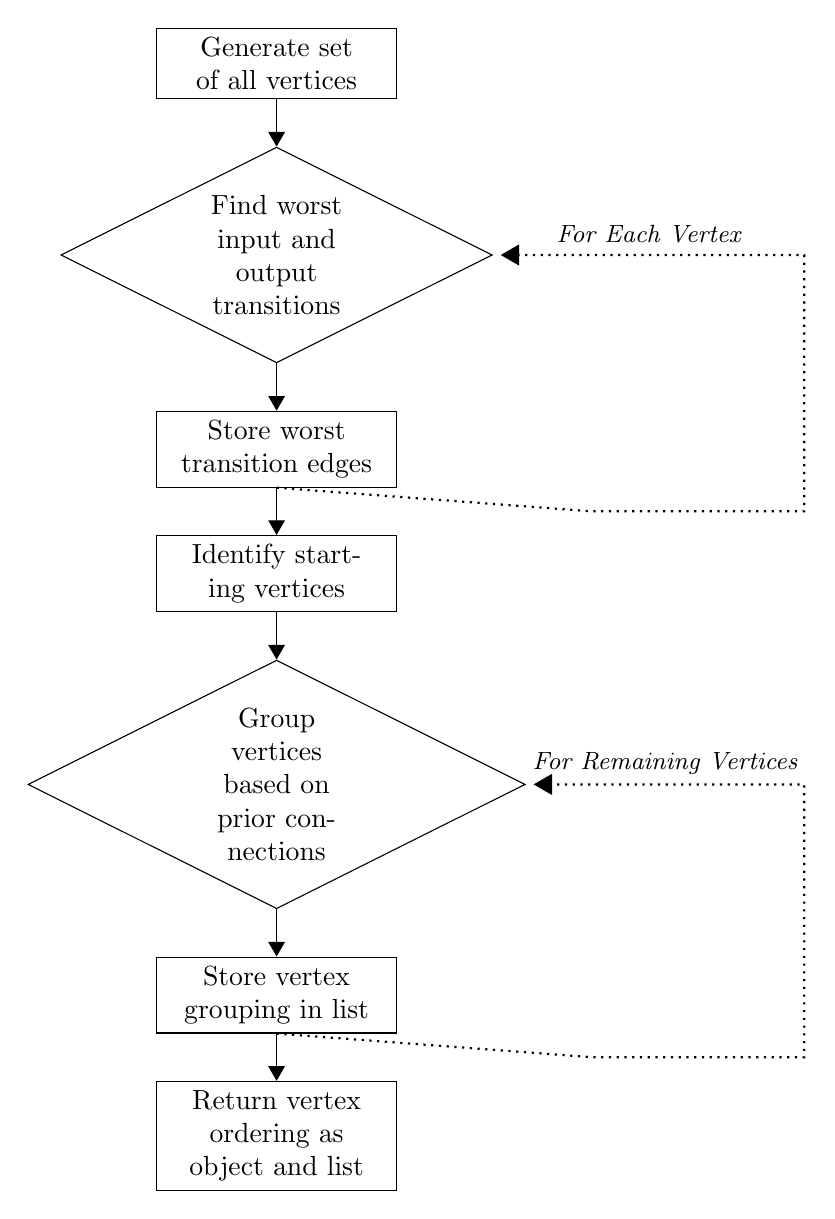
\begin{tikzpicture}[%
    >=triangle 60,              % Nice arrows; your taste may be different
    start chain=going below,    % General flow is top-to-bottom
    node distance=6mm and 60mm, % Global setup of box spacing
    every join/.style={norm},   % Default linetype for connecting boxes
    ]
% ------------------------------------------------- 
% A few box styles 
% <on chain> *and* <on grid> reduce the need for manual relative
% positioning of nodes
\tikzset{
  base/.style={draw, on chain, on grid, align=center, minimum height=4ex},
  proc/.style={base, rectangle, text width=8em},
  test/.style={base, diamond, aspect=2, text width=5em},
  % Connector line styles for different parts of the diagram
  norm/.style={->, draw},
  it/.style={font={\small\itshape}}
}
% -------------------------------------------------
% Start by placing the nodes
\node [proc] (p0) {Generate set of all vertices};
% Use join to connect a node to the previous one 
\node [test, join] (p1) {Find worst input and output transitions};
\node [proc, join] (p2) {Store worst transition edges};
\node [proc, join] (p3) {Identify starting vertices}; 
\node [test, join] (p4) {Group vertices based on prior connections};
\node [proc, join] (p5) {Store vertex grouping in list};
\node [proc, join] (p6) {Return vertex ordering as object and list};

\draw [->, dotted, thick, shorten >=1mm]
  (p2.south) -- ++(40mm,-3mm)  -- ++(27mm,0) 
  |- node [black, near end, yshift=0.75em, it]
    {For Each Vertex} (p1);
\draw [->, dotted, thick, shorten >=1mm]
  (p5.south) -- ++(40mm,-3mm)  -- ++(27mm,0) 
  |- node [black, near end, yshift=0.75em, it]
    {For Remaining Vertices} (p4);

% -------------------------------------------------
\end{tikzpicture}
}
	\caption{High Level Vertex Order Generation}
	\label{fig:node ordering}
\end{figure}

\noindent The process flow in defining the vertex ordering for the vertices is
listed in detail below:

\begin{description}
    \item[Vertex Ordering Generation:]
\end{description}
 \begin{enumerate}
   \item Generate set of all vertices
   \item For each vertex in set:
   \begin{enumerate}
     \item Initialize transitional weight to 0.
     \item For each element of the graph edge list:
     \begin{enumerate}
       \item Check if vertex matches the input vertex.
       \item Check if the number of transitions to the vertex is greater than the
       transitional weight.
       \item If both checks are true; set the transitional weight to the current
       list line's number of transitions.
       \item Also, if both checks are true; store this list line.
     \end{enumerate}
     \item After the worst input transition is found for the vertex, store it in
     the heavy edges set.
     \item Repeat this entire step for the output vertices.
   \end{enumerate}
   \item For each heavy edge element, search the graph edge list
   for input vertices that are also destination vertices.
   \begin{enumerate}
     \item Any vertices not found are set as start vertices.
     \item Repeat this step for output vertices that are also starting vertices. 
     Any vertices not found are set as ending vertices.
   \end{enumerate}
   \item Add all the starting vertices to vertex 0 and add them to the vertex store
   set.
   \item Add all vertices that are not starting vertices to the remaining
   vertices set.
   \item Increment the group number to 1.
   \item Until the remaining vertices set is empty, loop through the following
   steps.
   \begin{enumerate}
     \item For each vertex in vertex store, store all destination vertices in a
     set that vertex in vertex store transitions to.
     \item For each destination vertex stored in the previous step, find all
     possible next destination vertices and check if they are contained within
     the set generated in the previous step.
     \begin{enumerate}
       \item If one is contained within the previously generated set, remove
       the vertex from the set.
     \end{enumerate}
     \item Add remaining vertices to next vertex grouping.  Also remove remaining
     vertices from remaining vertices set.
     \item Add the vertex group to the vertex return list.
     \item Increment the group number.
     \item Replace the vertices in the starting vertices set with the vertices
     that were just added to a group.
   \end{enumerate} 
   \item Generate an object containing an array of the vertex groupings from
   the vertex return list.
   \item Return both the object and the vertex return list.
 \end{enumerate}



\subsection{Vertex Details}
Presenting all of the potential information would overwhelm any user interface,
so instead many of the details are buried within each vertex and can be queried
by the end user, by selecting the vertex of interest.  As each vertex contains
additional details such as the place of employment or education, time spent at
the school or job, or any other vertex relevant pieces of information; the data
must be gathered upon user request, as to not slow down the overall graph
generation.  Once the request is made, the data about the individuals who
reached the goal vertex and the data about all of the users who passed through a
particular vertex are pulled.  This data is then broken down into a statistic for
both cases and compared against each other to determine if something occurred
more frequently for the users who reached the goal vertex versus those who had
not.  This way any significant differences could be raised to the end user's
attention as potentially important steps to reaching the final goal.  The high
level process to generating this data is depicted in Figure~\ref{fig:node
details}.

\usetikzlibrary{shapes,arrows,chains}

\begin{figure}[H]
	\centering
% Start the picture
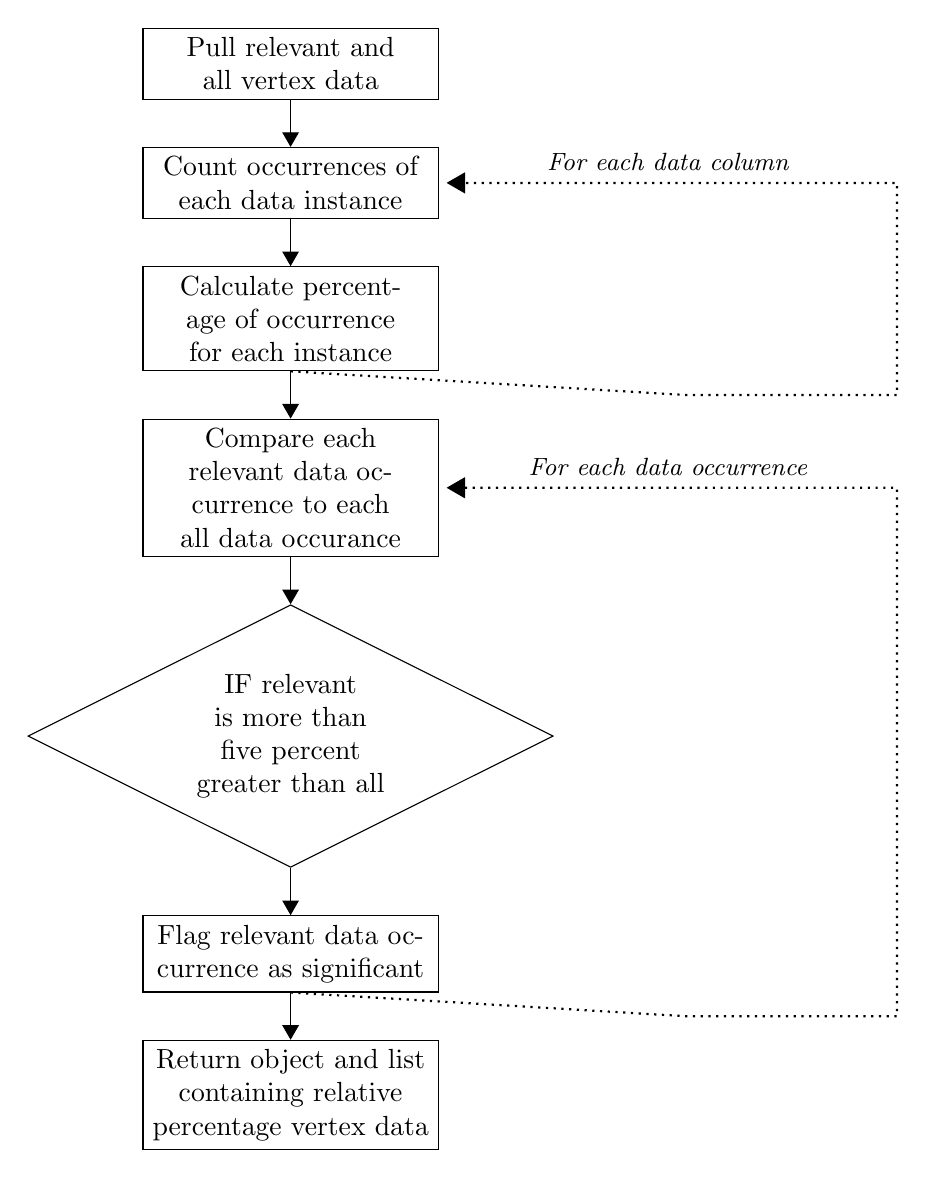
\begin{tikzpicture}[%
    >=triangle 60,              % Nice arrows; your taste may be different
    start chain=going below,    % General flow is top-to-bottom
    node distance=6mm and 60mm, % Global setup of box spacing
    every join/.style={norm},   % Default linetype for connecting boxes
    ]
% ------------------------------------------------- 
% A few box styles 
% <on chain> *and* <on grid> reduce the need for manual relative
% positioning of nodes
\tikzset{
  base/.style={draw, on chain, on grid, align=center, minimum height=4ex},
  proc/.style={base, rectangle, text width=10em},
  test/.style={base, diamond, aspect=2, text width=8em},
  % Connector line styles for different parts of the diagram
  norm/.style={->, draw},
  it/.style={font={\small\itshape}}
}
% -------------------------------------------------
% Start by placing the nodes
\node [proc] (p0) {Pull relevant and all vertex data};
% Use join to connect a node to the previous one 
\node [proc, join] (p1) {Count occurrences of each data instance};
\node [proc, join] (p2) {Calculate percentage of occurrence for each
instance};
 \node [proc, join] (p3) {Compare each relevant data occurrence to each all data
 occurance};
 \node [test, join] (t0) {IF relevant is more than five percent greater than
 all};
 \node [proc, join] (p4) {Flag relevant data occurrence as significant};
 \node [proc, join] (p5) {Return object and list containing relative percentage vertex data};

\draw [->, dotted, thick, shorten >=1mm]
  (p2.south) -- ++(50mm,-3mm)  -- ++(27mm,0) 
  |- node [black, near end, yshift=0.75em, it]
    {For each data column} (p1);
\draw [->, dotted, thick, shorten >=1mm]
  (p4.south) -- ++(50mm,-3mm)  -- ++(27mm,0) 
  |- node [black, near end, yshift=0.75em, it]
    {For each data occurrence} (p3);

% -------------------------------------------------
\end{tikzpicture}
	\caption{High Level Vertex Detail Generation}
	\label{fig:node details}
\end{figure}
\pagebreak

\noindent The process flow in defining the details and significant details for
each vertex is listed in detail below:

\begin{description}
    \item[Vertex Detail Generation:]
\end{description}
\begin{enumerate}
  \item Pull in profile list, tag each element as a profile, and then add
  the element to the complete list.
  \item Repeat this for the jobs list and the education list.
  \item Check each element of the complete list.
  \begin{enumerate}
    \item If the element contains the vertex that details are being pulled on, add
    the element to the relevant list.
  \end{enumerate}
  \item Pull the headers associated with the vertex that details are being pulled
  from.
  \item Pull all the data in the database for that vertex and store in the all
  vertex data list.
  \item For each element of the complete list:
  \begin{enumerate}
    \item Split the element into columns and step through each column.
    \begin{enumerate}
    	\item Check if the column element is a start or end year and instead
    	calculate the years spent at the vertex.
    	\begin{enumerate}
    	  \item If the end year is set to current, find the current year and then
    	  calculate the total years spent at the vertex.
    	\end{enumerate}
    	\item Add the column value to a set to obtain all possible values for
    	the column.
    	\item Step through the column counting each value instance to obtain a
    	count for each different value.
    	\item Calculate the percentage for each value in the column by diving the
    	count by the total number of elements.
    	\item Push these values into the relevant list.
    \end{enumerate} 
  \end{enumerate}
  \item Repeat for each element of the all vertex data list
  \item Compare the percentages for each element of the relevant list to
  the percentages from the all vertex data list.
  \begin{enumerate}
    \item Flag the column value for any instance where the relevant value's
    percentage exceeds the percentage for all the data by 5\%.
    \item Return this value as relevant so that it can be identified to the user
    as significant to the vertex.
  \end{enumerate}
  \item Return the relevant list and an object containing an array
  of the same data.
\end{enumerate}
\pagebreak

